% Patrick Donnelly
\documentclass[10pt, xcolor={table}]{beamer}
%------------------------------------------------
% Oregon State University
% by Patrick Donnelly
% Last Updated: 11/20/2022
%-----------------------------------------------

%------------------------------------------------
% Beamer Theme
%-----------------------------------------------
\usetheme[block=fill]{metropolis}

%------------------------------------------------
% Packages to Include
%-----------------------------------------------
\usepackage{appendixnumberbeamer}
\usepackage{color}
\usepackage{booktabs}
\usepackage[scale=2]{ccicons}
\usepackage{xcolor}
\usepackage{hyperref}
    \hypersetup{
        colorlinks=true,
        citecolor=beaver,
        linkcolor=beaver,
        filecolor=beaver,      
        urlcolor=beaver,
        }
    \urlstyle{same}
\usepackage{multimedia}
\usepackage{media9}   % If embedding sound/video
\usepackage{pgfplots}
\usepackage{ragged2e}
\usepackage{multicol}
\usepackage{multirow}
\usepgfplotslibrary{dateplot}
\usepackage{xspace}
\usepackage{fancyvrb}
\usepackage{listings}
\usepackage{etoolbox}% >= v2.1 2011-01-03
\usepackage{xpatch}
\usepackage[algoruled, noline, noend]{algorithm2e}
%\usepackage[utf8]{inputenc}
\usepackage[algoruled, noline]{algorithm2e}
\usepackage{ragged2e}
\usepackage{animate}
\usepackage[normalem]{ulem}
\usepackage{cancel}
\usepackage{subfigure}

%===========
% Variables
%===========

%-------------
% Logo Graphic 
%-------------
% OSU, OSUC, or Soundbendor
\def \logoOSUC {OSU-cascades}
\def \logoOSUhor {OSU-horizontal}
\def \logoOSUver {OSU-vertical}
\def \logoSoundbendor {Soundbendor}
\def \figPath {sty/logo/}   % path to logos
\def \logoWidth {0.4}        % OSU logo width (default 0.4)
\def \labWidth  {0.3}       % lab logo width (default 0.25)

% Campus: Corvallis or Cascades
\newcommand*{\campus}[1]{%
    \def\param{#1}%
    \def\corvallis{Corvallis}%
    \def\cascades{Cascades}%
    \ifx\param\corvallis
      % Corvallis
      \def\logoOSU{\logoOSUhor}
    \else
      % Cascades
      \def\logoOSU{\logoOSUC}
    \fi
}

%-----------------
% Title Page Logos
%-----------------
% Mode: Research or Teaching
\newcommand*{\presentmode}[1]{%
    \def\param{#1}%
    \def\research{research}
    \def\teaching{teaching}
    
    \ifx\param\teaching
    %\def\titleResearch{0}  
    % Title slide for Teaching: hide lab logo
    \titlegraphic{
        \vspace{6.5cm}
        \hfill\includegraphics[width=\logoWidth\textwidth]{\figPath\logoOSU}
    }
    \else
    \def\titleResearch{1}
    % Title slide for Research: show lab logo
    \titlegraphic{
        \begin{tikzpicture}[remember picture,overlay]
        \node[opacity=0.9,anchor=north east,xshift=-10pt,yshift=-5pt] at (current page.north east) {\includegraphics[height=15mm]{\figPath\logoOSU}};
        \end{tikzpicture}

        % lab, bottom centered
        \begin{tikzpicture}[remember picture,overlay]
          \node[opacity=0.8,anchor=south,xshift=0pt,yshift=0pt] at (current page.south) {
\includegraphics[height=15mm]{sty/logo/soundbendor.png}};
        \end{tikzpicture}
        }

    % Frame Bottom Left: Soundbendor Lab (Research)
    \addtobeamertemplate{frametitle}{}{%
        \begin{tikzpicture}[remember picture,overlay]
          \node[opacity=0.6,anchor=south west,xshift=4pt,yshift=0pt] at (current page.south west) {
\includegraphics[height=8mm]{sty/logo/soundbendor.png}};
        \end{tikzpicture}}        
    \fi
}

%----------------
% Frame Page Logo
%----------------

% Top Right: OSU vertical
\addtobeamertemplate{frametitle}{}{%
    \begin{tikzpicture}[remember picture,overlay]
      \node[opacity=0.8,anchor=north east,xshift=-8pt,yshift=0pt] at (current page.north east) {
\includegraphics[height=7mm]{sty/logo/OSU-vertical-white.png}};
    \end{tikzpicture}}

%-----------------
% Useful Operators
%-----------------
\DeclareMathOperator*{\argmin}{argmin}
\DeclareMathOperator*{\argmax}{argmax}
\newcommand*{\argminl}{\argmin\limits}
\newcommand*{\argmaxl}{\argmax\limits}

%=======================
% Template Modifications
%=======================
\newcommand{\themename}{\textbf{\textsc{metropolis}}\xspace}
\setbeamercolor{frametitle}{fg=white,bg=beaver!90}
\setbeamercolor{title separator}{fg=beaver}
\setbeamercolor{alerted text}{fg=solarflare}
\setbeamertemplate{caption}{\raggedright\insertcaption\par} % remove word Figure 

%-----------
% OSU Colors
%-----------
\definecolor{beaver}{HTML}{D73F09}
%   paddletail black = 000000
%   bucktooth white = FFFFFF
% Secondary - normal
\definecolor{pinestand}{HTML}{4A773C}
\definecolor{hightide}{HTML}{00859B}
\definecolor{luminance}{HTML}{FFB500}
\definecolor{stratosphere}{HTML}{006A8E}
% Secondary - light
\definecolor{reindeermoss}{HTML}{C4D6A4}
\definecolor{seafoam}{HTML}{B8DDE1}
\definecolor{candela}{HTML}{FDD26E}
\definecolor{moondust}{HTML}{C6DAE7}
% Secondary - dark
\definecolor{hopbine}{HTML}{AA9D2E}
\definecolor{roguewave}{HTML}{0D5257}
\definecolor{solarflare}{HTML}{D3832B}
\definecolor{starcanvas}{HTML}{003B5C}
% Secondary - grays
\definecolor{till}{HTML}{B7A99A}
\definecolor{coastline}{HTML}{A7ACA2}
\definecolor{highdesert}{HTML}{7A6855}
\definecolor{crater}{HTML}{8E9089}

%-------
% Blocks 
%-------
\setbeamertemplate{blocks}[rounded][shadow=true]   % rounded

% Example block
\setbeamercolor{block title example}{fg=pinestand} 
\setbeamerfont{block title example}{series=\bfseries} 
% Alter block
\setbeamercolor{block title alerted}{fg=beaver} 
\setbeamerfont{block title alerted}{series=\bfseries} 

%------------
% Code Blocks
%------------
\lstset{language=C++,
		basicstyle=\scriptsize\ttfamily,
		abovecaptionskip=0pt,belowcaptionskip =6pt,
		framextopmargin=-\topsep, 
                      keywordstyle=\color{stratosphere}\bfseries,
		morekeywords={},
		%literate={\&}{{\CodeSymbol{\&}}}1{**}{{\CodeSymbol{**}}}1,
	  stringstyle=\color{solarflare}\bfseries,
        commentstyle=\color{pinestand}\bfseries,        
		%morecomment=[l][\color{brown}]{\#},
	    showstringspaces=false,
	    escapechar=\@
     }


%------------------
% Frame environment
%------------------
\usetikzlibrary{shadows}
\usepackage[%
    framemethod=tikz,
    skipbelow=\topskip,
    skipabove=\topskip
]{mdframed}
\mdfsetup{%
    leftmargin=0pt,
    rightmargin=0pt,
	shadow=true,
	shadowsize=5pt,
    backgroundcolor=coastline!20,
    middlelinecolor=gray,
    roundcorner=6
}
\BeforeBeginEnvironment{lstlisting}{\begin{mdframed}\vspace{-0.2em}}
\AfterEndEnvironment{lstlisting}{\vspace{-0.5em}\end{mdframed}}

\makeatletter
\gdef\lst@commenttypes{l,L,f,s,n}
\gdef\lst@CommentDM@L#1#2#3\@empty#4#5#6{%
    \lst@CArg #2\relax\lst@DefDelimB{}{}{}#4{#1}{#6\lst@Lmodetrue}%
    \lst@CArg #3\relax\lst@DefDelimE{}{}{}#5{#1}}
\makeatletter

\newmdenv[innerlinewidth=0.5pt, roundcorner=4pt,linecolor=starcanvas,innerleftmargin=6pt,
innerrightmargin=6pt,innertopmargin=6pt,innerbottommargin=6pt]{roundbox}

%----------------
% Itemize spacing 
%----------------
% Enum letters not numbers			
\renewcommand{\theenumi}{\Alph{enumi}}

\setlength\leftmargini  {2em}
\setlength\leftmarginii {2em}
\setlength\leftmarginiii{2em}
\setlength  \labelsep   {.5em}
\setlength  \labelwidth{\leftmargini}
\addtolength\labelwidth{-\labelsep}

\def\@listi{\leftmargin\leftmargini
            \topsep -4\p@ \@plus0\p@ \@minus0\p@
            \parsep 0\p@
            \itemsep0\p@ \@plus0\p@ \@minus0\p@}
\let\@listI\@listi

% TODO Need to change sizes at level 2 and 3
\def\@listii{\leftmargin\leftmarginii
              \topsep    2\p@ \@plus1\p@ \@minus2\p@
              \parsep    0\p@   \@plus\p@
              \itemsep   \parsep}
\def\@listiii{\leftmargin\leftmarginiii
              \topsep    2\p@ \@plus1\p@ \@minus2\p@
              \parsep    0\p@   \@plus\p@
              \itemsep   \parsep}  
        

%-------------
% Bullet shape 
%-------------
\def \bulletcolor {beaver!90}
\setbeamertemplate{items}[circle]
\setbeamercolor{item}{fg=\bulletcolor} 
\setbeamercolor{description item}{fg=\bulletcolor} 

\defbeamertemplate{itemize item}{squarealt}%
{\tiny\raise.5ex\hbox{\donotcoloroutermaths\color{\bulletcolor}$\blacksquare$}}
\defbeamertemplate{itemize subitem}{squarealt}%
  {\tiny\raise.4ex\hbox{\donotcoloroutermaths$\triangleright$}}
\defbeamertemplate{itemize subsubitem}{squarealt}%
  {\tiny\raise.3ex\hbox{\donotcoloroutermaths$\square$}}
  
\defbeamertemplate{itemize item}{circlealt}%
  {\small\raise.2ex\hbox{\donotcoloroutermaths$\bullet$}}
\defbeamertemplate{itemize subitem}{circlealt}%
  {\small\raise.1ex\hbox{\donotcoloroutermaths$\circ$}}
  \defbeamertemplate{itemize subsubitem}{circlealt}%
{\scriptsize\raise.1ex\hbox{\donotcoloroutermaths$\bullet$}}
\def\circletext{circle}

\ifx\beamer@fancy@bullet\circletext
  \setbeamertemplate{items}[circlealt]
\else
  \setbeamertemplate{items}[squarealt]
\fi

%-------------------------
% Overlay Support
%-------------------------
% strikethrough
\renewcommand<>{\sout}[1]{\alt#2{\beameroriginal{\sout}{#1}}{#1}}


%-------------------------
% Algorithm2e (pseudocode)
%-------------------------
% Change 
\SetAlFnt{\small\sf}
\SetAlCapFnt{\small\sf}
\SetAlCapNameFnt{\small\sf}

%\SetAlFnt{\footnotesize\sf}
\newcommand{\mykeywordsty}[1]{\textbf{\textcolor{stratosphere}{#1}}}
\SetKwSty{mykeywordsty}
%\SetFuncSty{mykeywordsty}
%\SetFuncArgSty{mykeywordsty}

\renewcommand{\thealgocf}{}
\linespread{1.0}\selectfont
\NoCaptionOfAlgo
\DontPrintSemicolon

\SetKwInOut{Input}{inputs}
\SetKwInOut{Local}{local}
\SetKwInOut{Output}{output}
\SetKwProg{Fn}{function}{}{}
\SetKwProg{Unless}{unless}{\ do}{}
\SetKwProg{Repeat}{repeat until}{\ do}{}





%--------------------
% Additional Packages
%--------------------
% Note: many common packages added by osu.tex
% add other packages here 
% ...


%===========
% Variables
%===========
% Campus (Pick one!)
    \campus{Corvallis}   % choose Corvallis
    %\campus{Cascades}   %    or Cascades logo

% Presentation type (Pick one!)
    \presentmode{research}  % choose Research
    %\presentmode{teaching}   %   or Teaching mode

% Set values (if Teaching mode)
\def\courseID{CS XXX}
\def\courseName{Course Name}
\def\term{Spring 202X}
\def\professor{Professor}

%===========
% Title Page
%===========
\title{Title}             % <== set Title

\ifdef{\titleResearch}{
    % RESEARCH
    \subtitle{Subtitle}   % <== set Subtitle
    \author{Author}       % <== set Author
    \date{\today}  
}{
    % TEACHING, set the variables above
    \subtitle{\courseID - \courseName}  
    \author{\professor}
    \date{\term}    
}

\begin{document}
\maketitle

%========================================================
%  Block Example
%========================================================
\begin{frame}{Block Example}
    % Regular block
    \begin{block}{Block Title}
    Some block text. 
    \end{block}
    % Example block
    \begin{example}
    Some example text. 
    \end{example}
    % Definition block
    \begin{definition}
    Some definition text. 
    \end{definition}
    % Alert block
    \begin{alertblock}{Alert Block Title}
    Some alertblock text. 
    \end{alertblock}
\end{frame}


%========================================================
% List Example
%========================================================
\begin{frame}{List Examples}
    \begin{columns}[]
    \column{5cm}  % left column
        \begin{enumerate}
        \item enum default one
        \item enum default two
        \item enum default three
        \end{enumerate}
        \bigskip\bigskip
        
        \begin{enumerate}[a]
        \item enum alpha one
        \item enum alpha two
        \item enum alpha three
        \end{enumerate}
        \bigskip\bigskip
        
        \begin{enumerate}[I]
        \item enum roman one
        \item enum roman two
        \item enum roman three
        \end{enumerate}
    
     \column{5cm}   % right column
        \begin{itemize}
        \item item one
        \begin{itemize}
        \item subitem one
        \begin{itemize}
        \item subsubitem one
        \item subsubitem two
        \item subsubitem three
        \end{itemize}
        \item subitem two
        \item subitem three
        \end{itemize}
        \item item two
        \item item three
        \end{itemize}
        \bigskip\bigskip
    
        \begin{description}[align=left]
        \item[label1] description one
        \item[label2] description two
        \item[label3] description three
        \end{description}
    \end{columns}
\end{frame}

%========================================================
% OSU Colors
%========================================================
\newcommand{\legendbox}[1]{%
  \textcolor{#1}{\rule{\fontcharht\font`X}{\fontcharht\font`X}}%
}

\begin{frame}{OSU Colors}

    \begin{columns}[]
    \column{3cm}
        \legendbox{beaver} \quad \textbf{\textcolor{beaver}{Beaver}} \\ \bigskip
        \legendbox{black} \quad \textbf{\textcolor{black}{Paddletail}} \\ \bigskip
        \legendbox{pinestand} \quad \textbf{\textcolor{pinestand}{Pine Stand}} \\\bigskip
        \legendbox{hightide} \quad \textbf{\textcolor{hightide}{High Tide}} \\\bigskip
        \legendbox{luminance} \quad \textbf{\textcolor{luminance}{Luminance}} \\ \bigskip
        \legendbox{stratosphere} \quad \textbf{\textcolor{stratosphere}{Stratosphere}} \\ \bigskip        
    \column{3cm}
        \legendbox{reindeermoss} \quad \textbf{\textcolor{reindeermoss}{Reindeer Moss}} \\ \bigskip
        \legendbox{seafoam} \quad \textbf{\textcolor{seafoam}{Seafoam}} \\ \bigskip
        \legendbox{candela} \quad \textbf{\textcolor{candela}{Candela}} \\ \bigskip
        \legendbox{moondust} \quad \textbf{\textcolor{moondust}{Moondust}} \\ \bigskip
        \legendbox{hopbine} \quad \textbf{\textcolor{hopbine}{Hop Bine}} \\ \bigskip
        \legendbox{roguewave} \quad \textbf{\textcolor{roguewave}{Rogue Wave}} \\ \bigskip
    \column{3cm}
        
        \legendbox{solarflare} \quad \textbf{\textcolor{solarflare}{Solar Flare}} \\ \bigskip
        \legendbox{starcanvas} \quad \textbf{\textcolor{starcanvas}{Star Canvas}} \\ \bigskip
        \legendbox{till} \quad \textbf{\textcolor{till}{Till}} \\ \bigskip
        \legendbox{coastline} \quad \textbf{\textcolor{coastline}{Coastline}} \\ \bigskip
        \legendbox{highdesert} \quad \textbf{\textcolor{highdesert}{High Desert}} \\ \bigskip
        \legendbox{crater} \quad \textbf{\textcolor{crater}{Crater}} \\ \bigskip
    \end{columns}	
\end{frame}

%========================================================
% Two Column Example
%========================================================
\begin{frame}{Two Column Example}
    \begin{columns}[]
    \column{5cm}
        \begin{center}
        \textbf{Column One} 
        \end{center}
        \begin{table}[h]
        \rowcolors{2}{beaver!15}{white} 
        \begin{tabular}{|r|r|}
        \hline
        \rowcolor{beaver!90}
        \color{white} $\mathbf{n}$&\color{white} $\mathbf{n!}$\\\hline \hline
        1&1\\
        2&2\\
        3&6\\
        4&24\\
        5&120\\
        6&720\\
        7&5040\\
        8&40320\\
        9&362880\\
        10&3628800\\
        \hline
        \end{tabular}
        \caption{This is a table.}
        \end{table}
        \vfill
    \column{5cm}
        \begin{center}
        \textbf{Column Two} \\\bigskip
        \end{center}
        \begin{center}
        \begin{figure}
        	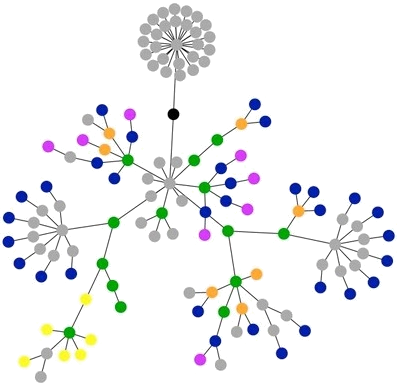
\includegraphics[width=0.95\textwidth]{img/graphic}
        	\caption{This is a figure.}
        \end{figure}
        \end{center}
        \medskip    
    \end{columns}	
\end{frame}


%========================================================
%  Formula Examples
%========================================================
\begin{frame}{Formula Example}
    \small
    \begin{eqnarray*}
        \frac{1}{n}\sin x & = & \mathrm{?} \\
        \frac{1}{\cancel{n}} \mathrm{si}\cancel{\mathrm{n}} ~x & = & \mathrm{?} \\
        \mathrm{six} & = & 6
    \end{eqnarray*}
    \bigskip
    
    \hspace{12mm} Expand $(a+b)^n$:  \vspace{-7mm}
    \begin{gather*}
      (a + b)^n\\
      (a\ + \ b)^n\\
      (a\quad + \quad b)^n\\
      (a\qquad + \qquad b)^n
    \end{gather*}
    \bigskip
    
    \begin{center}
    $
    \begin{bmatrix}
        \cos 90^{\circ} & \sin 90^{\circ}\\
       -\sin 90^{\circ} & \cos 90^{\circ}
    \end{bmatrix}
    \begin{bmatrix} a1 \\ a2 \end{bmatrix}
    =
    $
    \rotatebox[origin=c]{270}{$\begin{bmatrix} a1 \\ a2 \end{bmatrix}$}
    \end{center}
    \bigskip
\end{frame}



%========================================================
%  Listings Example
%========================================================
\begin{frame}[fragile]{Syntax Highlighting Example }
    %\vspace{-5mm}
    \begin{center}
    \begin{minipage}[t]{0.5\textwidth}
    \begin{lstlisting}[basicstyle=\tiny]
    /******  A Love Poem in C  ******/
    char*lie;
        double time, me= !0XFACE,
        not; int rested, get, out;
        main(ly, die) char ly,**die ;{
            signed char lotte,
    
    dear; (char)lotte--;
        for(get= !me;; not){
        1 -  out & out ;lie;{
        char lotte, my= dear,
        **let= !!me *!not+ ++die;
            (char*)(lie=
        
    "The gloves are OFF this time,   
        I detest you, snot\n\0sed GEEK!");
        do {not= *lie++ & 0xF00L* !me;
        #define love (char*)lie -
        love 1s *!(not= atoi(let
        [get -me?
             (char)lotte-            ...
    \end{lstlisting}
    \end{minipage}
    \\\bigskip
    \href{http://www.ioccc.org/1990/westley.c}{A Love Poem in C}, by Brian Westley (1990)
    \end{center}
\end{frame}


%========================================================
%  TIKZ Example
%========================================================
\begin{frame}{tikz Example}
    \def\layersep{2.5cm}
    \begin{center}
    \begin{tikzpicture}[shorten >=1pt,->,draw=black!50, node distance=\layersep]
        \tikzstyle{every pin edge}=[<-,shorten <=1pt]
        \tikzstyle{neuron}=[circle,fill=black!25,minimum size=17pt,inner sep=0pt]
        \tikzstyle{input neuron}=[neuron, fill=starcanvas];
        \tikzstyle{output neuron}=[neuron, fill=pinestand];
        \tikzstyle{hidden neuron}=[neuron, fill=luminance];
        \tikzstyle{annot} = [text width=4em, text centered]
    
        % Draw the input layer nodes
        \foreach \name / \y in {1,...,4}
        % This is the same as writing \foreach \name / \y in {1/1,2/2,3/3,4/4}
            \node[input neuron, pin=left:Input \#\y] (I-\name) at (0,-\y) {};
    
        % Draw the hidden layer nodes
        \foreach \name / \y in {1,...,5}
            \path[yshift=0.5cm]
                node[hidden neuron] (H-\name) at (\layersep,-\y cm) {};
    
        % Draw the output layer node
        \node[output neuron,pin={[pin edge={->}]right:Output}, right of=H-3] (O) {};
    
        % Connect every node in the input layer with every node in the
        % hidden layer.
        \foreach \source in {1,...,4}
            \foreach \dest in {1,...,5}
                \path (I-\source) edge (H-\dest);
    
        % Connect every node in the hidden layer with the output layer
        \foreach \source in {1,...,5}
            \path (H-\source) edge (O);
    
        % Annotate the layers
        \node[annot,above of=H-1, node distance=1cm] (hl) {Hidden layer};
        \node[annot,left of=hl] {Input layer};
        \node[annot,right of=hl] {Output layer};
    \end{tikzpicture}
    \end{center}
\end{frame}


%========================================================
% Sound File  Example
%========================================================
\begin{frame}{Embedding a Sound File}
    \begin{center}
     \href{http://www.haverford.edu/computerscience/resources/songs/}{\textbf{Loop Invariants}}\\ by \textit{J.P. Dougherty} \\
    
    \bigskip

    \includemedia[
    addresource=media/loop-invariants.mp3,
    flashvars={
    source=media/loop-invariants.mp3
    &autoPlay=true
    },
    transparent,
    passcontext %show APlayer's right-click menu
    ] 
    {\color{beaver}\framebox[0.25\linewidth][c]{Play}}{APlayer.swf}

    
    %\includemedia[
    %  addresource=snd/loop-invariants.wav,
    %  flashvars={
    %    source=snd/loop-invariants.wav
    %   &autoPlay=true
    %  }
    %]{\fcolorbox{white}{beaver}{\color{white}Play}}{APlayer.swf}
    \end{center}
    
    \bigskip
    
    \begin{columns}[]
    \footnotesize
    \it
     \column{5cm}
    Loop invariants, loop invariants\\
    Keep me on the road,\\
    Loop invariants, loop invariants\\
    As I write my code.\\
    \bigskip
    Preconditions, postconditions,\\
    Help to shed some light.\\
    Assertions used to write the loop\\
    Will help me get it right.
     \column{5cm}
    Loop invariants, loop invariants\\
    They can be a pain.\\
    Loop invariants, loop invariants\\
    Oh, but what I gain.\\
    \bigskip
    Executing, substituting,\\
    Each does complement.\\
    Code correctness is the goal\\
    Of loop invariants.
    \end{columns}
    \bigskip
\end{frame}


%========================================================
%  Blank Frame  
%========================================================
{
 \setbeamercolor{background canvas}{}
 \usebackgroundtemplate{ }

\begin{frame}[plain]{}
    This is how to implement a blank frame.
\end{frame}
}


\end{document}